\documentclass[a4paper,12pt]{article}
\usepackage{amsmath}
\usepackage{graphicx}
\usepackage{amssymb}
%\usepackage{hyperref}

% Renewed commands
\renewcommand{\Re}{\mathrm{Re}}
\renewcommand{\Im}{\mathrm{Im}}
\renewcommand{\mod}[1]{\left|#1\right|}
\renewcommand{\vec}[1]{\mathbf{#1}}

% New commands
\newcommand{\sqmod}[1]{\left|#1\right|^{2}}

% Formatting short-cuts
\newcommand{\rmi}{\mathrm{i}}
\newcommand{\rme}{\mathrm{e}}
\newcommand{\E}{\epsilon}

% Dirac notation
\newcommand{\bra}[1]{\left<#1\right|}
\newcommand{\ket}[1]{\left|#1\right>}

\newcommand{\iprod}[2]{\left<#1|#2\right>}
\newcommand{\iprodM}[3]{\left<#1\right|#2\left|#3\right>}

\newcommand{\oprod}[2]{\left|#1\right>\left<#2\right|}
\newcommand{\oprodM}[3]{\left|#1\right>#2\left<#3\right|}

\newcommand{\up}{\uparrow}
\newcommand{\down}{\downarrow}



\begin{document}

\title{Unequal Pumping - Investigations}

\author{M.P. Vaughan and M.J. Adams}

\date{\today}

\maketitle

%*******************************************************************************************
\section{Zero detuning}
%*******************************************************************************************

Investigation of the stability boundaries for unequal pumping using

\begin{equation}
\mod{\eta} = \frac{\alpha_{H}\left(Q_{A} + Q_{B} - 2\right)\left(1-q^{2}\right)^{3/2}}{2\tau_{p}\left[\left(Q_{A}+Q_{B}\right)\left(1 - q^{2}\right) + 2q^{2}\right]}, \label{eq:inphase}
\end{equation}

\noindent delimiting in-phase stable solutions and 

\begin{equation}
\mod{\eta} = \frac{\left[\left(Q_{A} + Q_{B}\right)\left(1 - q^{2}\right) + 2q^{2}\right]\left(1-q^{2}\right)^{1/2}}{4\alpha_{H}\tau_{N}}, \label{eq:antiphase}
\end{equation}

\noindent for the anti-phase solutions, where

\begin{equation}
q = \frac{Q_{A} - Q_{B}}{Q_{A} + Q_{B} -2}. \nonumber
\end{equation}

\noindent In the limiting case $Q_{A} = Q_{B} = Q$, these reduce to the Wingful-Wang expressions

\begin{equation}
\mod{\eta} = \frac{\alpha_{H}\left(Q-1\right)}{2\tau_{p}Q} \label{eq:WW_inphase}
\end{equation}

\noindent and 

\begin{equation}
\mod{\eta} = \frac{Q}{4\alpha_{H}\tau_{N}}, \label{eq:WW_antiphase}
\end{equation}

\noindent respectively.

In the following, we allow $\eta$ and $Q_{A}$ to vary keeping the remaining parameters listing in Table~\ref{table1} fixed. For these calculations, we choose $Q_{B} = 20$.


\begin{table}[h!]
\centering 
\begin{tabular}{ll}
Parameter & Value \\
\hline
alpha  &  5 \\
cavity loss rate (1/ns) &  200 \\
carrier loss rate (1/ns) & 1 \\
coupling (equal) & varied \\
coupling phase (rad) & 0 \\
detuning (rad/ns) & 0 \\
pump (A) & varied \\
pump (B) & 20 \\
\hline \\
\end{tabular}

\begin{tabular}{llll}
Axis & Parameter & Start & End \\
\hline
$X$ & pump (A) & 2 & 40  \\ 
$Y$ & coupling (equal) & 1 & 2000  \\ 
\hline
\end{tabular}

\caption{Stability map calculation data (set 1).}\label{table1}

\end{table}

\begin{figure}[h!]
\centering 
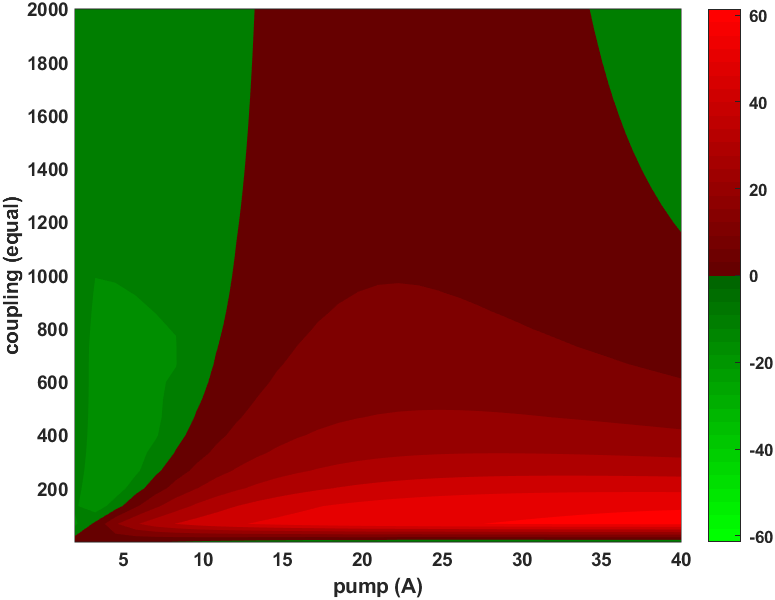
\includegraphics[width=0.8\textwidth]{Eq_10_antiphase_large_QB_20.png}
\caption{Stability map for parameters in Table~\ref{table1} for \emph{anti-phase} solutions on a large scale (there are no expressions applicable for this region).}
\end{figure}


\begin{figure}[h!]
\centering 
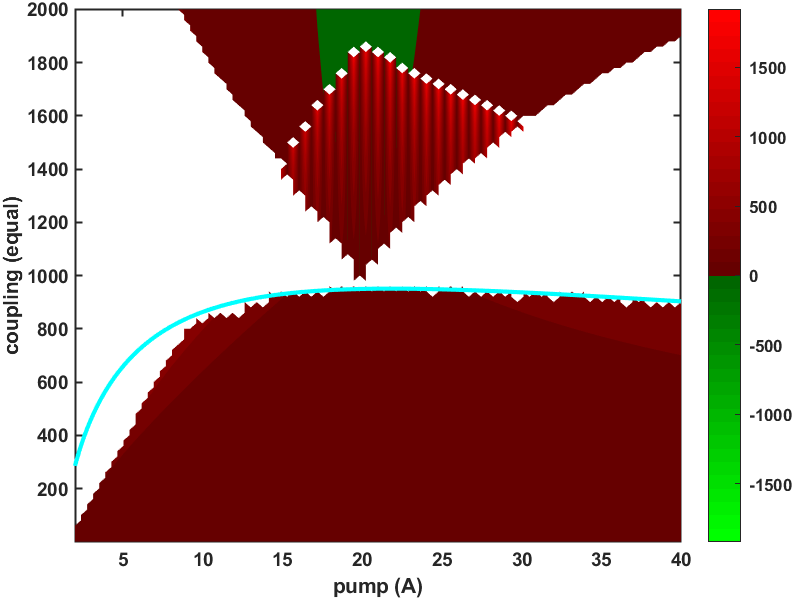
\includegraphics[width=0.8\textwidth]{Eq_10_inphase_QB_20.png}
\caption{Stability map for parameters in Table~\ref{table1} for \emph{in-phase} solutions. The cyan curve shows Eq.~\eqref{eq:inphase}. Note that no stable, in-phase solutions were found in this region by the stability mapper.}
\end{figure}


\begin{table}[h!]
\centering 
\begin{tabular}{llll}
Axis & Parameter & Start & End \\
\hline
$X$ & pump (A) & 2 & 40  \\ 
$Y$ & coupling (equal) & 0.01 & 4  \\ 
\hline
\end{tabular}

\caption{Small scale range for $\eta$.}\label{table2}

\end{table}

\begin{figure}[h!]
\centering 
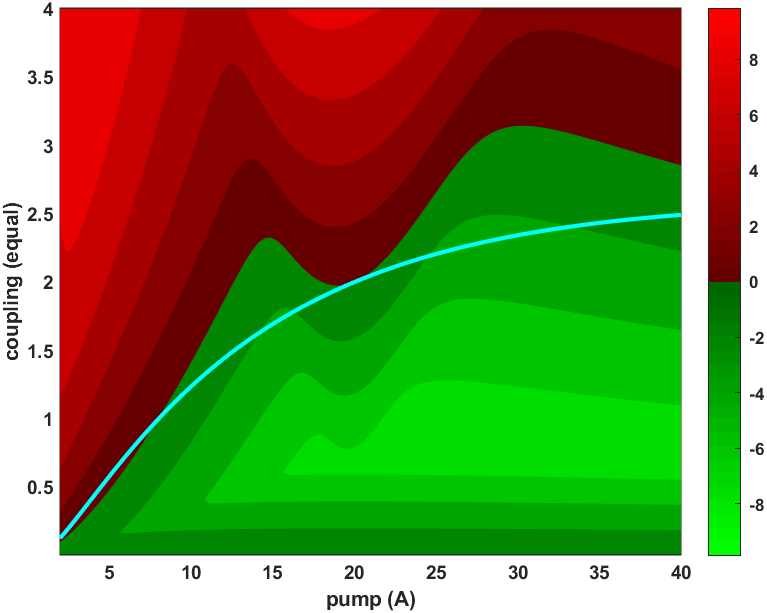
\includegraphics[width=0.8\textwidth]{Eq_10_antiphase_small_QB_20.png}
\caption{Stability map for ranges in Table~\ref{table2} for \emph{anti-phase} solutions. The cyan curve is for Eq.~\eqref{eq:antiphase}. The curve bears little relation to the map, although both coincide at $Q_{A} = 20$ when Eq.~\eqref{eq:antiphase} reduces to the Wingful-Wang expression Eq.~\eqref{eq:WW_antiphase}.}
\end{figure}




%\bibliographystyle{unsrt}
%\bibliography{bib_file}


\end{document}